
\section{Heaven}\label{sec:impl-intro}

The architecture of the \textsc{Test Stand} consists in three stand alone modules that establish a mono-directional communication flow: \textsc{Streamer}, \textsc{RSP Engine} and \textsc{Result Collector}. Some of the requirements reported in Section \ref{sec:requirements} directly affect the implementation experience of \name and Chapter \ref{chap:heaven} describes how fulfil them. First of all the requirements [R.10], i.e. the need of an \textit{Extendible Design}, and [R.11], which states the necessity of an \textit{Event-base architecture} to properly face any RSPEngine, are immediately relevant. 

To be \textit{Extendible} the \textsc{Test Stand} requires two main abstractions: the \textit{Event} and the \textit{EventProcessor}.

\textit{Event} concept is required to build a hierarchical communication. Indeed, the \textsc{Test Stand} may handle three events flows: one internal to the RSP Engine module, one for the communication between modules and one to communicate with the user. Next section about data clarifies the communication structured. 

The \textit{Event Processor} guarantees the system to be modular, it standardizes the interaction simplifying the behaviour of each component in the system. 

Thus, a module is an \textit{Event Processor} which can be positioned everywhere in the the \textsc{Test Stand} pipeline. % As a matter of facts, specific implementations of a module may reduce the generality of this definition and also the flexibility of the module itself.	

\begin{figure}[tbh]
  \centering
	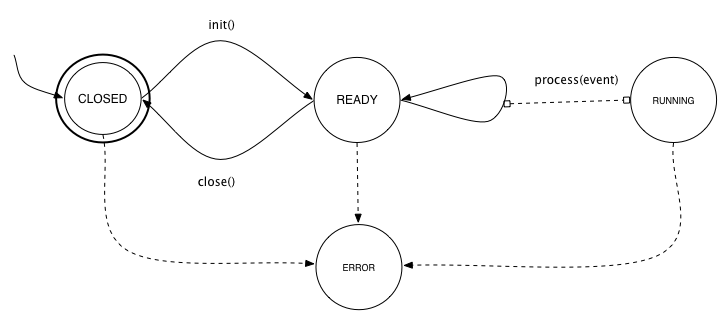
\includegraphics[width=\linewidth]{images/fsm-schema}
	\caption{Module Finite State Machine Automata} 
  	\label{fig:module-fsm}
\end{figure}

The requirement [R.4] states the \textsc{Test Stand} \textit{must not be running when the RSP Engine is under execution} (see Section \ref{sec:requirements}) conditioning \name workflow. To cover [R.4] we designed the status of each module  as a Finite State Machine (FSM), which can work only in those states that allow processing (READY). The schema in Figure \ref{fig:module-fsm} represents the FSM for each module of \name, even the Baselines, and also for the \textsc{Test Stand} external structure. 
A modules moves from CLOSED state to READY with a standard initialisation method. We state that each module is an \textit{EventProcessor} and the \textit{ process (Event e)} brings the module into RUNNING state until the processing ends, and then back to READY. One and only one module can be in the RUNNING state in a certain moment during the execution. This behaviour is exploited by the \textsc{Test Stand} external structure to control execution fulfilling [R.4] by stopping its process while the RSPEngine is running (see Section \ref{sec:teststand}). ERROR State, which can be reached from any point of the execution, prevents the propagation of errors over result data: when a module fails the execution is stopped without saving the erroneous data (last event) and reporting the error to the user.


\section{Events and Data}\label{sec:data-impl}

Chapter \ref{chap:problem-settings} poses the requirements of an Event-based architecture [R.11] for the \textsc{Test Stand}. Moreover, Chapter \ref{chap:heaven} describes \name workflow and how it exchanges events during the execution. The \textsc{Test Stand} modules interact trough events, see \ref{fig:uml_events},  which contains data at different points of the experiment process. \name handles three kind of events:

\begin{figure}[tbh]
  \centering
	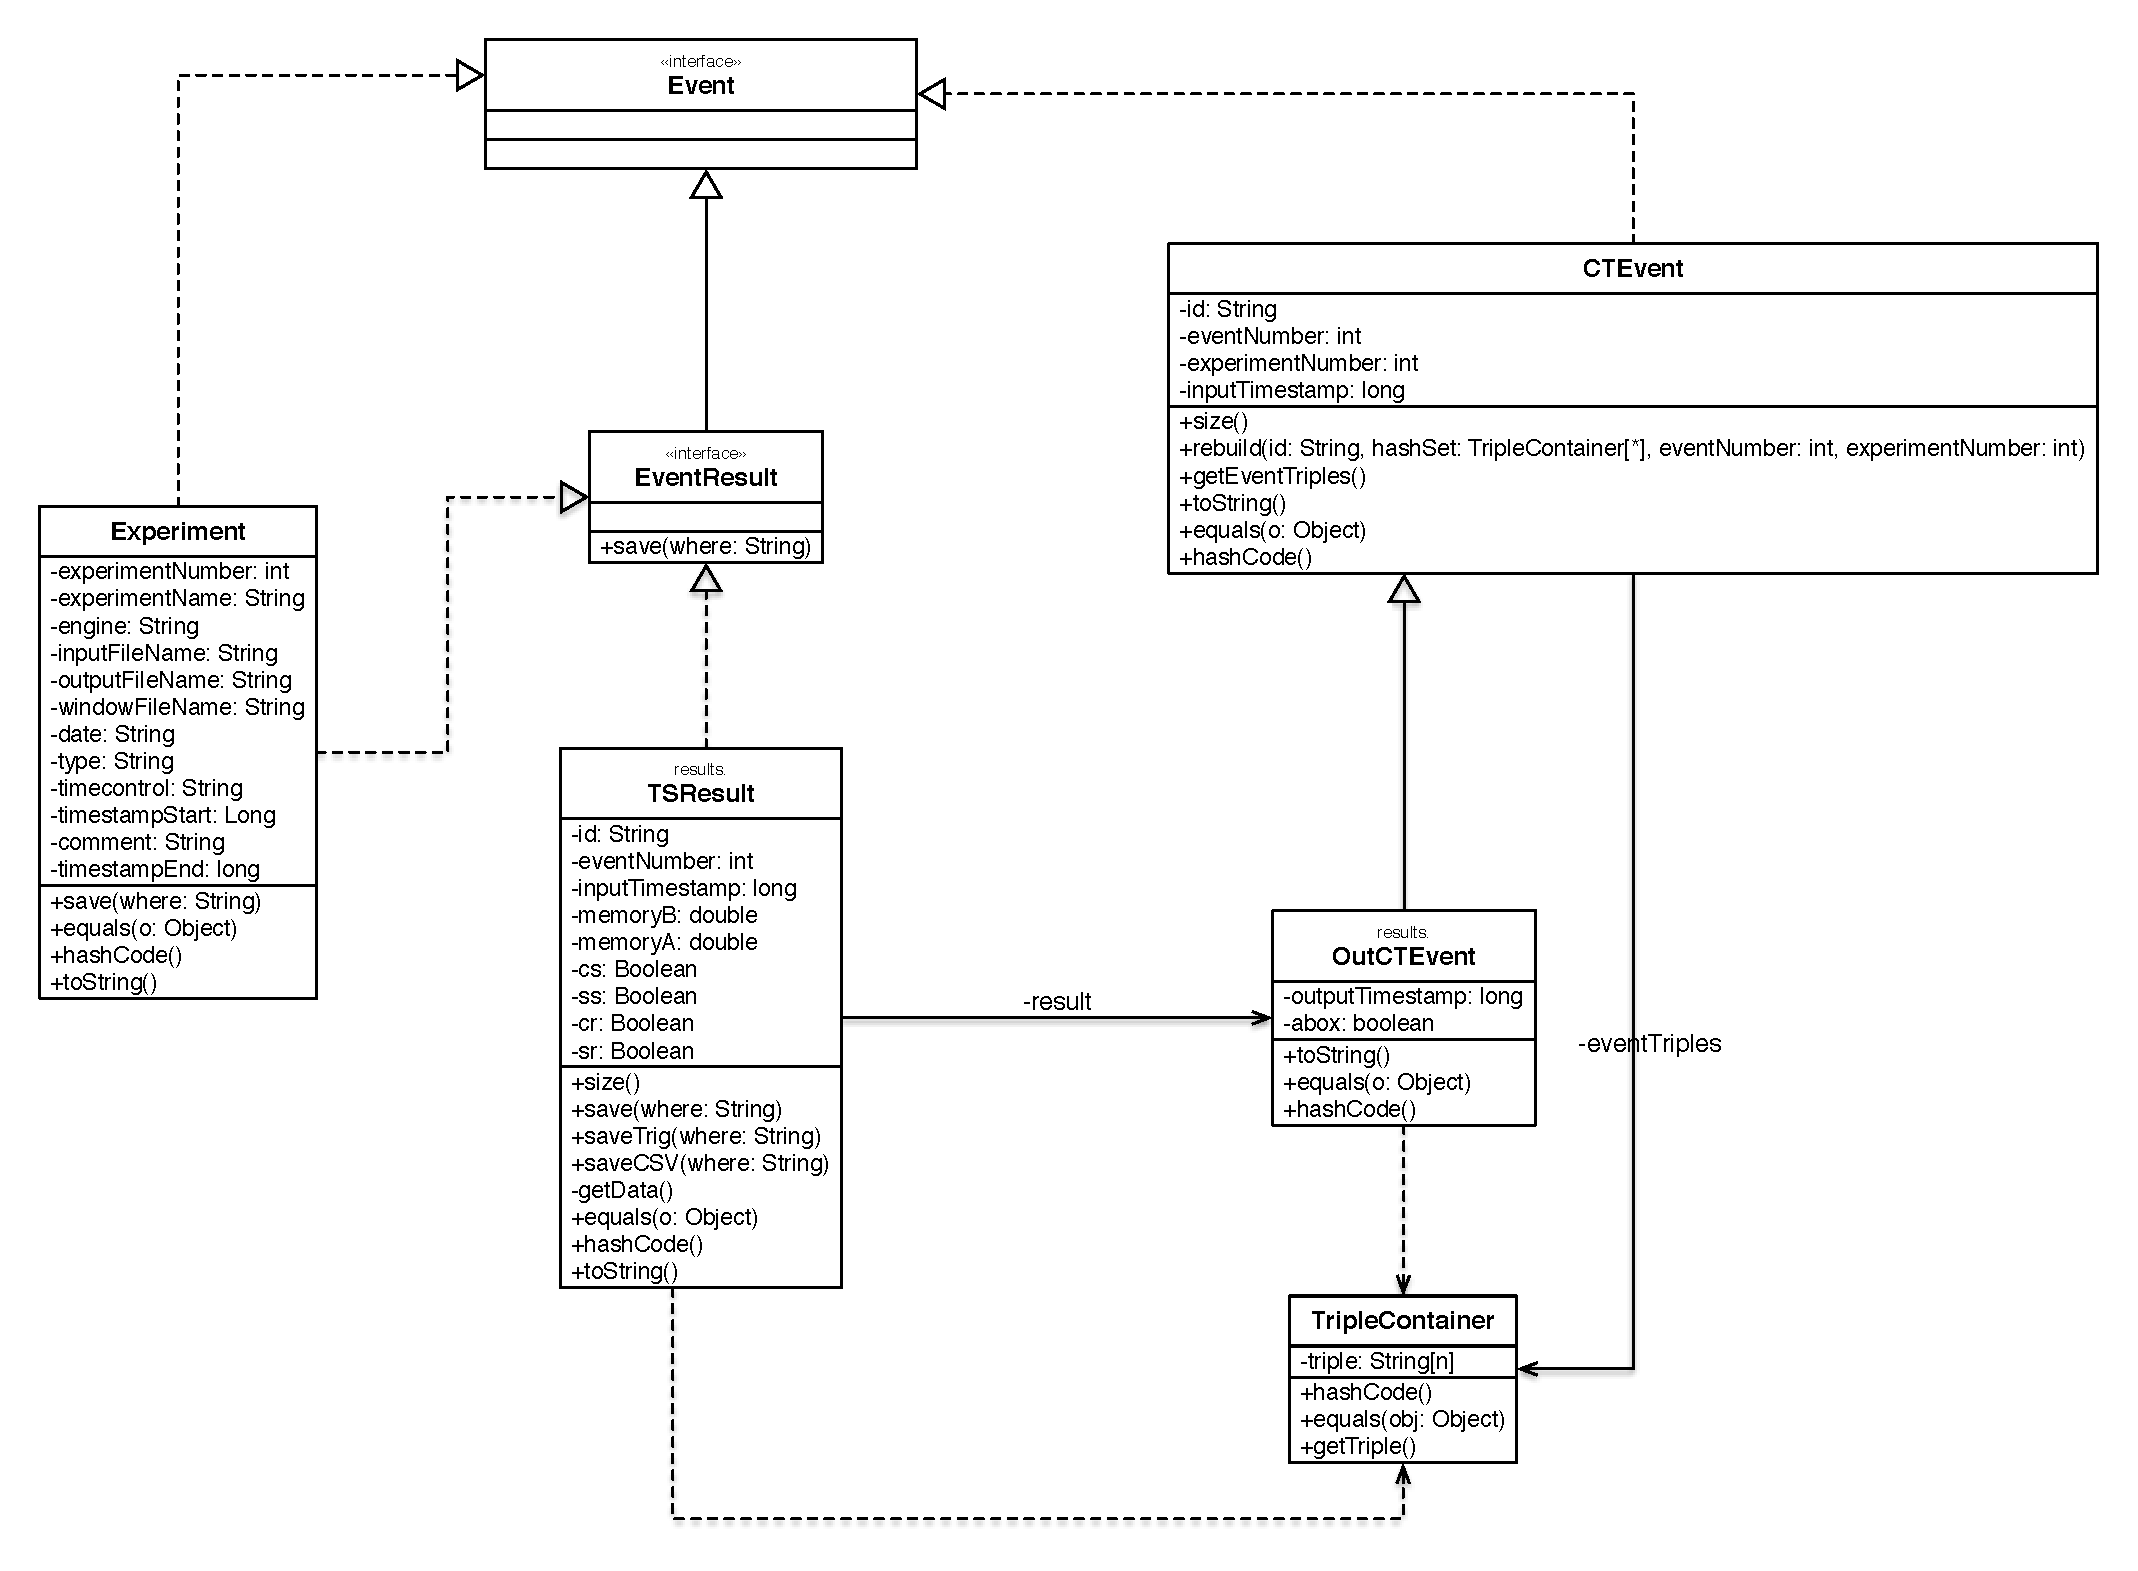
\includegraphics[width=\linewidth]{images/uml_events}
	\caption{UML Schema for all the events involved in the system} 
  	\label{fig:uml_events}
\end{figure}

\begin{itemize}
\item \textit{Experiment} - it represents the tuple $<\mathcal{E}, \mathcal{D},\mathcal{T},\mathcal{Q}>$ and all the experiment metadata like start time or end time.
\item \textit{CTEvent and OutCTEvent} - they contains a set of triples which has the same timestamp. The \textit{OutCTEvent} represents the event produced by the RSPEngine after processing the active window. Figure \ref{fig:uml_events} show the inheritance relation between \textit{CTEvent} and \textit{OutCTEvent}
\item \textit{TSResult} - it wraps the \textit{OutCTEvent} adding the information about the minimal sensor data: memory and latency and complete and soundness if it evaluated at runtime (see Section \ref{sec:requirements})
\end{itemize}

\name requires an initialization phase to prepare the \textit{Experiment} and provide it to the \textsc{Test Stand}. The current implementation exploits a property file with the Experiment parameters: ID and the tuple $<\mathcal{E}, \mathcal{D},\mathcal{T},\mathcal{Q}>$. 

The \textit{CTEvent} and the \textit{OutCTEvent} contain RDF triples in NT-Triple\footnote{http://www.w3.org/2001/sw/RDFCore/ntriples/}, which is the easiest RDF serialisation to parse. This serialisation was chosen to fulfil requirement [R.12], which demands an \textit{Easy-to-Parse RDF Serialisation for the events presented to the RSP Engine in exam}. Figure \ref{fig:uml_events} shows also that the RDF Triples are stored in the events into the \textit{TripleContainer} wrapper: we redefine the triple hashcode and equals method guaranteeing their uniqueness of within an \textit{CTEvent} or \textit{OutCTEvent}.

\section{Modules}

In Section \ref{sec:impl-intro} we define a module a an \textit{Event Processor} which can be positioned everywhere in the the \textsc{Test Stand} pipeline. Moreover, we introduce the FSM schema which describe a module lifecycle in \ref{fig:module-fsm}. We state that each module must be initialized to reach the READY state where the processing is allowed. 

The \textit{Startable} Interface standardize two methods, init() and close() which allow to control the behaviour of the Module at the start and the end of the execution. Notice that the ERROR state translate an exceptional behaviour which has to be handled exceptionally by each module, according with its internal mechanisms. 

In this section we present the three modules which compose \name: the \textsc{Streamer},  the \textsc{ResultCollector} and the  \textsc{Test Stand Supporting Structure}. They all extend the \textit{EventProcessor} concept and the \textit{Startable} interface, offering three standard method to interact with them: \textit{process(Event e)} from \textit{EventProcessor} and \textit{init()} and \textit{close()} from the \textit{Startable} Interface.

\subsection{Streamer}	\label{sec:streamer-impl}
\begin{figure}[tbh]
  \centering
	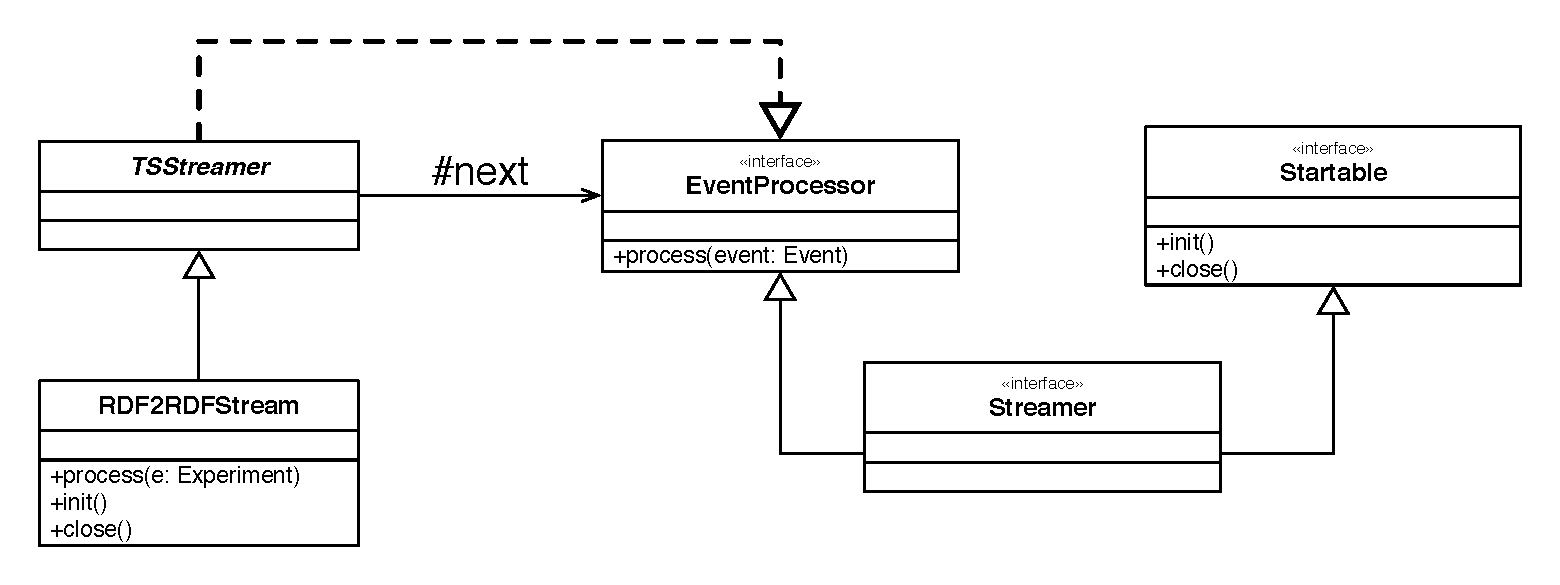
\includegraphics[width=\linewidth]{images/uml_tstreamer}
	\caption{Streamer UML Schema with TSStreamer and Implementation example} 
  	\label{fig:uml_tstreamer}
\end{figure}

The head-module in the \textsc{Test Stand} pipeline is the on \textit{TSStreamer}, see Figure \ref{fig:uml_tstreamer}, which is the most general implementation of the \textsc{Streamer}. The \textit{TSStreamer} processes an \textit{Experiment}, received by an external initialisation class. It and communicates, once initialized, with one referenced \textit{EventProcessor}, called \textit{next}, which process \textit{CTEvent} and follows in the pipeline. The nature of the communication between the\textit{TSStreamer} and the following \textit{EventProcessor} can follow the user needs, and passing different events. Notice that also the \textit{next} must be initialised before starting the communication, otherwise the ERROR state will be reached when the event is received by the \textit{next}, because the processing is not allowed.

Figure \ref{fig:uml_tstreamer} shows also the actual implementation, the \textit{RDF2RDFStream}, while in Figure \ref{fig:uml_flowrateprofiler} is presented its internal mechanism. 
The \textit{RDF2RDFStream} was developed to conduct experiments as they are presented in Chapter \ref{chap:evaluation}.  It is worth to note that we use LUBM Benchmarks to generate the data for the experiments. LUBM generated data are static, thus the \textit{RDF2RDFStream} builds an RDFStream attaching to the static data produced by LUBM a timestamp. The file is generated using  LUBM(1000,0), which means 1000 different universities with the random generation seed 0. 

\begin{figure}[tbh]
  \centering
	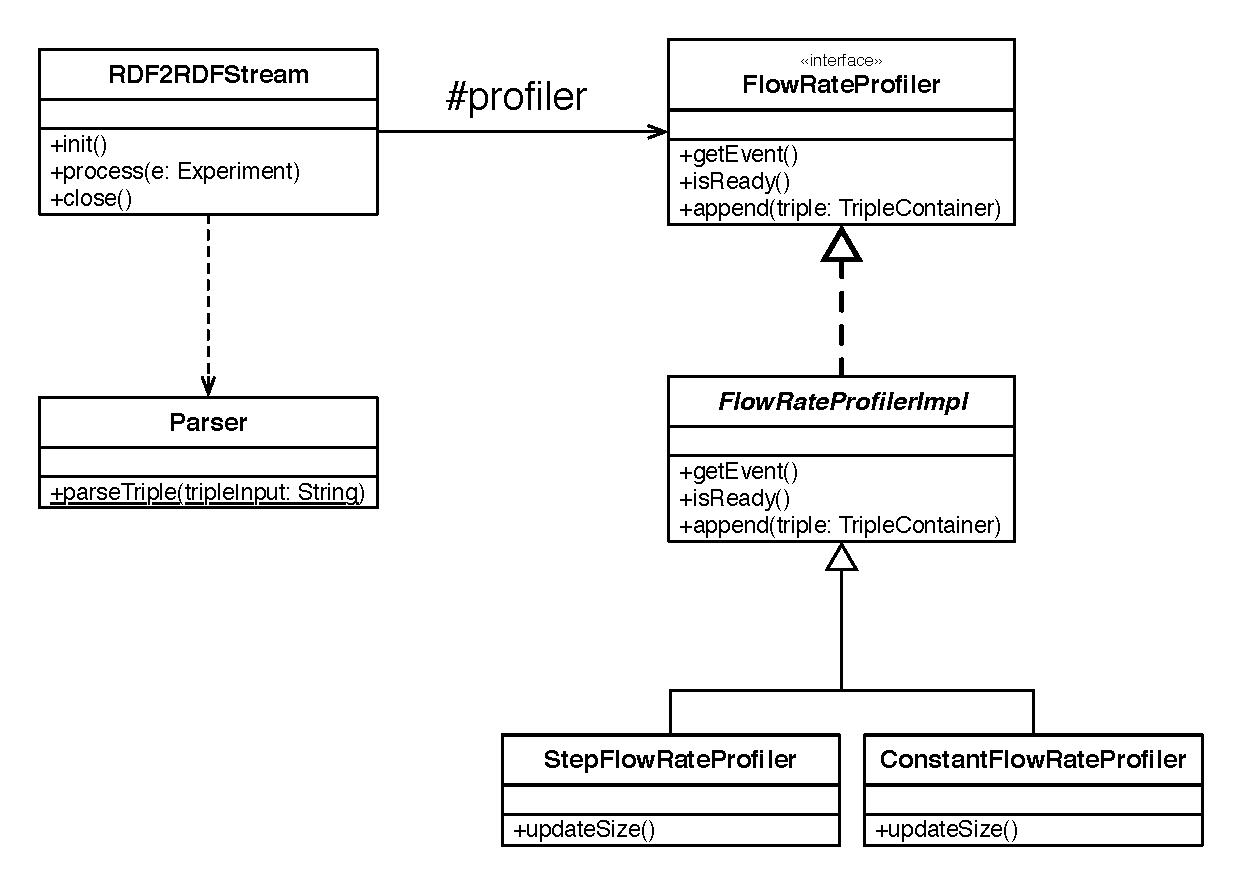
\includegraphics[width=0.75\linewidth]{images/uml_flowrateprofiler}
	\caption{RDF2RDFStream internal UML Schema} 
  	\label{fig:uml_flowrateprofiler}
\end{figure}


The \textit{Parser} component, in Figure \ref{fig:uml_flowrateprofiler} can be accessed statically by \name modules. It reads in memory one by one the triples in the file guaranteeing data independence [R.1] and it does not influence the memory footprint [R.5] by allocating only the memory necessary to parse a triple. 

Figure \ref{fig:uml_flowrateprofiler} also includes the \textit{FlowRateProfiler}. This component determines the number of triples to add to a \textit{CTEvent} and builds such an event. In this way, \textit{RDF2RDFStream} can generate different RDF streams $\mathcal{D}$, which differ on the number of contemporary triples in the stream. 

\begin{figure}[tbh]
\centering
\subfigure[Exponential Growing Size: $y=2^x$]{
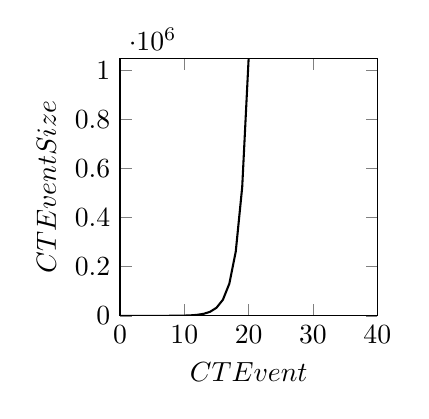
\begin{tikzpicture}
  \begin{axis}[ 
  width=0.4\linewidth,
      height=0.4\textwidth,
    xlabel=$CTEvent$,
    ylabel={$CTEvent Size$},
    xmin=0.00, xmax=40,
	ymin=0, ymax=1048576
  ] 
    \addplot [
    line width=0.75pt]
    coordinates {
    		(0.00, 1.00)
		(1.00, 2.00)
		(2.00, 4.00)
		(3.00, 8.00)
		(4.00, 16.00)
		(5.00, 32.00)
		(6.00, 64.00)
		(7.00, 128.00)
		(8.00, 256.00)
		(9.00, 512.00)
		(10.00, 1024.00)
		(11.00, 2048.00)
		(12.00, 4096.00)
		(13.00, 8192.00)
		(14.00, 16384.00)
		(15.00, 32768.00)
		(16.00, 65536.00)
		(17.00, 131072.00)
		(18.00, 262144.00)
		(19.00, 524288.00)
		(20.00, 1048576.00)
		};	
		
	\end{axis}
\normalsize

\end{tikzpicture}
}
\subfigure[Step Growing Size with K1=100 and K2=1000 after 9 CTEvents]{
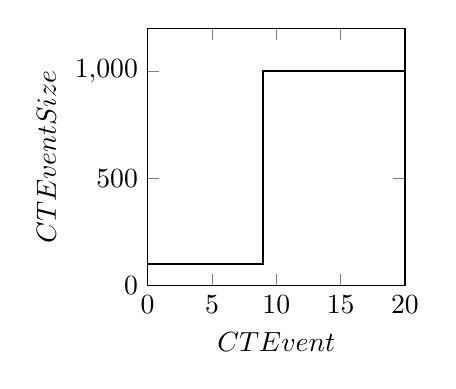
\begin{tikzpicture}
  \begin{axis}[ 
  width=0.4\linewidth,
      height=0.4\textwidth,
    xlabel=$CTEvent$,
    ylabel={$CTEvent Size$},
    xmin=0.00, xmax=20,
	ymin=0, ymax=1200
  ] 
    \addplot [
    line width=0.75pt]
    coordinates {
    		(0.00, 100.00)
		(1.00, 100.00)
		(2.00, 100.00)
		(3.00, 100.00)
		(4.00, 100.00)
		(5.00, 100.00)
		(6.00, 100.00)
		(7.00, 100.00)
		(8.00, 100.00)
		(9.00, 100.00)
		(9.00, 1000.00)
		(10.00, 1000.00)
		(11.00, 1000.00)
		(12.00, 1000.00)
		(13.00, 1000.00)
		(14.00, 1000.00)
		(15.00, 1000.00)
		(16.00, 1000.00)
		(17.00, 1000.00)
		(18.00, 1000.00)
		(19.00, 1000.00)
		(20.00, 1000.00)
		};	
		
	\end{axis}
\normalsize

\end{tikzpicture}
}
\caption{Example of CTEvent size growing by the FlowRateProfiler}
\label{fig:frp-examples}
\end{figure}


The \textit{FlowRateProfiler} builds the triple according to a function $y=f(x)$, in which $x$ is the number of the \textit{CTEvent} and it results that $y$ is the number of triple this \textit{CTEvent} will contain. 

Practically $f$ can be any function from N to N. For example if we decide to increase linearly the number of triples inside a \textit{CTEvent} the function $f$ will be: \[y=x, \text{ where } x,y \in N\]

The first event (E0) will contain zero triple, E1 will contain only one triple following E4 will contain four triples and so forth. Another possibility is to increase exponentially the number of triples inside a \textit{CTEvent} : \[y=2^x, \text{ where } x,y \in N\] 
The first event (E0) will contain one triple, E1 will contain two triple following E3 will contain eight triples and so forth, Figure \ref{fig:frp-examples}.a shows the resulting behaviour plotting the triple number on y-axis and \textit{CTEvent} number on x-axis

We develop two \textit{FlowRateProfiler} for our experiment: 
\begin{itemize}
\item \textit{ConstantFlowRateProfiler}, which maintains the same number of triples for each events over all the experiment: \\
\[y=K, \text{ where } K \in N \]

\item \textit{StepFlowRateProfiler}  which maintain a constant number of triple $K1$ inside a \textit{CTEvents} for $x$ events, specified in the set-up phase. When $x$ are created,  suddenly changes the number of triple $y$ form $K1$ to $K2$ where $K2 >> K1$. Figure \ref{fig:frp-examples}.b contains the resulting plot of implemented function which follows:

\[
y=
\begin{cases}
K1, &\text{if $x < M$ } $ where $ K1, M \in N\\
K2, &\text{if $x >= M$} $ where $ K2 >> K1, K2 \in N
\end{cases}
\]


\end{itemize}
Other implementations are available in \name right now, but are not used in the experiments:
\begin{itemize}
\item \textit{LinearStepFlowRateProfile}, which stream $x$ CTEvents of dimension $y$, in terms of triples, then linearly increase the number of a quantity $M$: \[y=x*M, \text{ where } x,y,M \in N\]
\item \textit{ConstantRandomFlowRateProfiler}, which changes $y$ and $x$ according with two random generators directed by two seeds. \[y=random(seed), \text{ where } random(seed),y \in N\]
\end{itemize}


\subsection{Result Collector} 

\noindent The \textsc{ResultCollector} is the acquisition system that collects the query results and the measurements data gathered by the \textsc{Test Stand} during the execution of an experiment.

\begin{figure}[tbh]
  \centering
	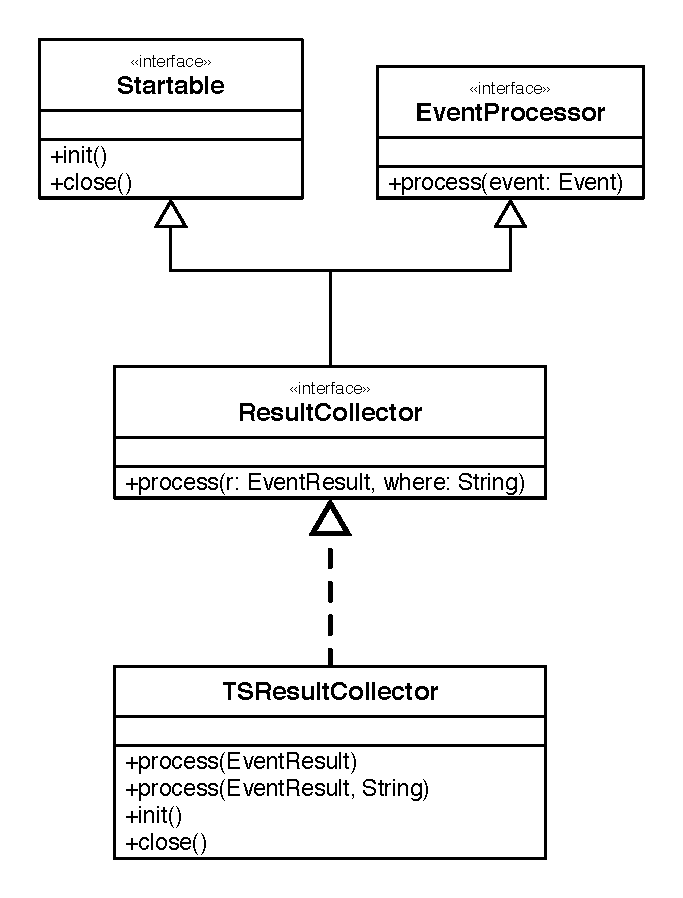
\includegraphics[width=\linewidth]{images/uml_resultcollector}
	\caption{ResultCollector UML Schema with events Experiment, TSResult and OutCTEvent} 
  	\label{fig:uml_resultcollector}
\end{figure}

The UML Schema in Figure \ref{fig:uml_resultcollector} shows the implementation of the \textit{ResultCollector} interface, named \textit{TSResultCollector}, which is again an \textit{EventProcessor}. The \textit{TSResultCollector} stays at the end position in the pipeline which composes the \textsc{Test Stand}. It is responsible of saving data in a way that is independent from which data format, since requirement [R.7] demands to \textit{enable users extensions with new software sensors and specific measurements collection}.  The general saving procedure exploits the \textit{EventResult} interface, which exposes methods to delegate the implementation of such a procedure to the provider of the event, according to his needs. Figure \ref{fig:uml_resultcollector} shows the relation between the \textit{EventResult} interface and the \textit{TSResultCollector}, which calls the exposed methods \textit{save(location)} over all the events passed to it during the execution. 


\begin{figure}[tbh]
  \centering
	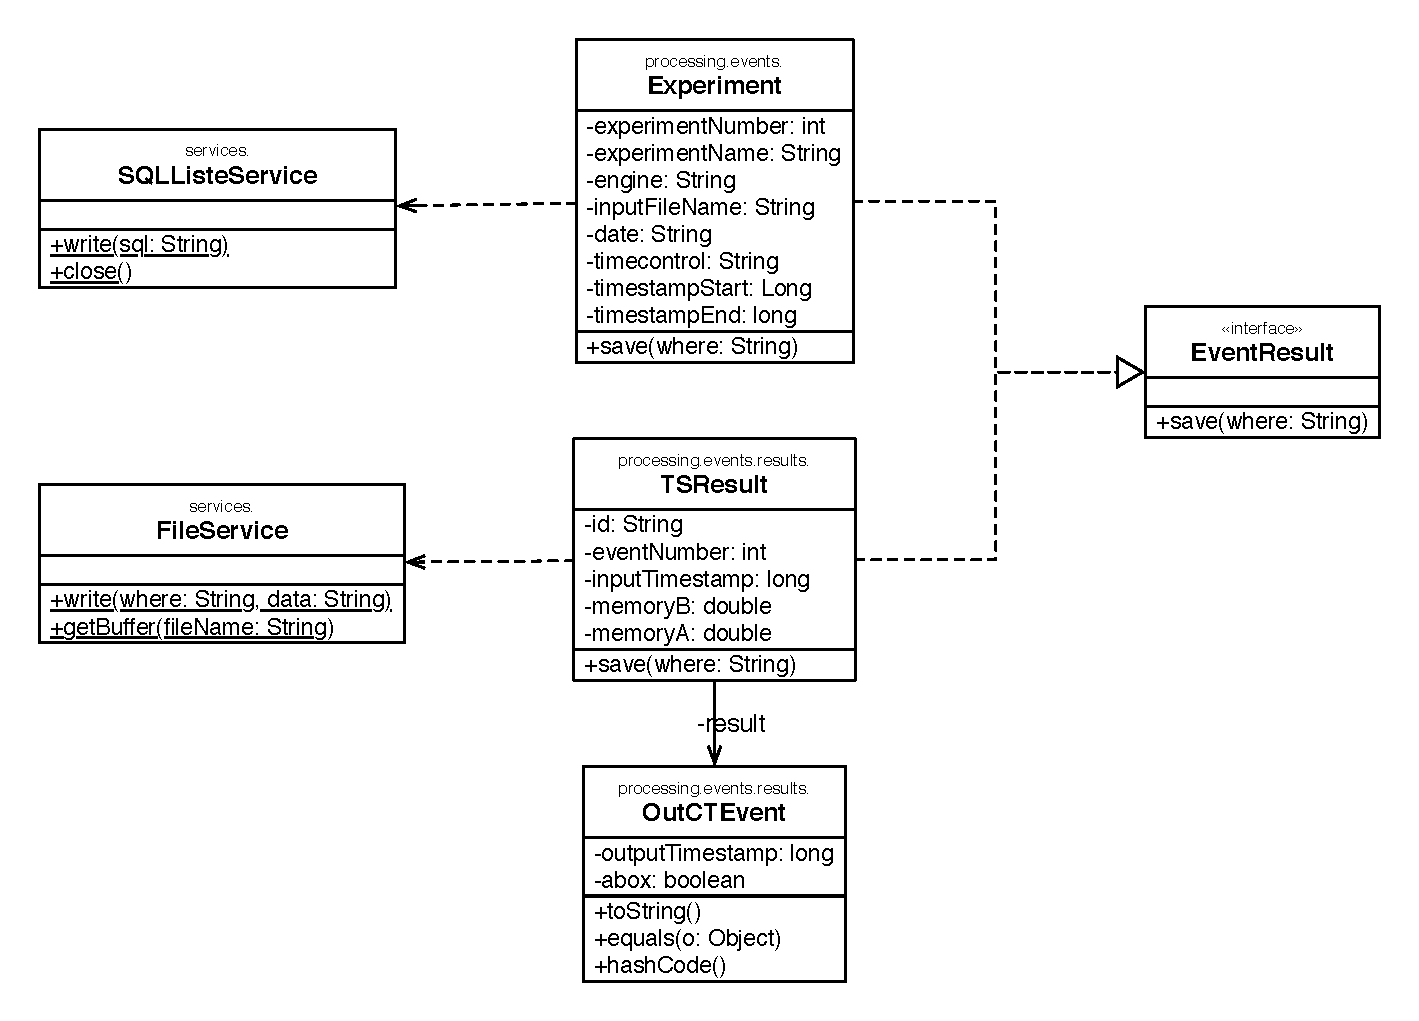
\includegraphics[width=\linewidth]{images/uml_resultcollector_events}
	\caption{ResultCollector events  UML Schema: Experiment, TSResult and OutCTEvent} 
  	\label{fig:uml_resultcollector_events}
\end{figure}

Moreover, Figure \ref{fig:uml_resultcollector_events}, shows how different events in the system exploit the \textit{EventResult} interface. In the current implementation the \textit{TSResultCollector} handles two kinds of event:
\begin{itemize}
\item \textit{TSResult} - it saves the data of the query results into a TriG\footnote{http://www.w3.org/TR/trig/} file where the graph name is the event id inside the experiment, while it save the sensor data with event id into a CSV\footnote{$http://en.wikipedia.org/wiki/Comma-separated_values$} file. 
\item \textit{Experiment}. It saves the experiment metadata and the tuple \\ $<\mathcal{E},\mathcal{D},\mathcal{T},\mathcal{Q}>$ collapsed into a generic description field into SQLite\footnote{https://sqlite.org/} database.
\end{itemize} 

The two saving procedure exploits service classes, the \textit{SQLLIsteService} and the \textit{FileService} in Figure \ref{fig:uml_resultcollector_events}, which exposes static methods to interact with the file-system. The goal is  reducing system complexity offering a single point to interact with the file-system, which usually is a slow operation, to avoid parallel interactions that may influence the experiment. 


\subsection{Test Stand Supporting Structure}\label{sec:teststand}


\begin{figure}[tbh]
  \centering
	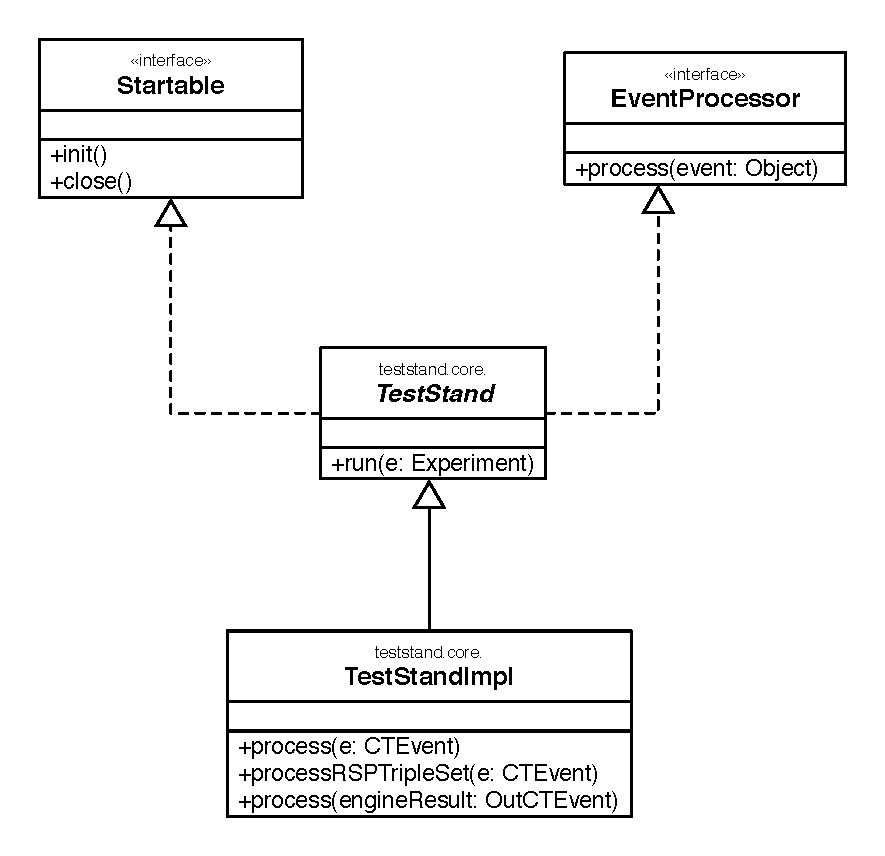
\includegraphics[width=\linewidth]{images/uml_teststand}
	\caption{UML Schema the TestStand} 
  	\label{fig:uml_teststand}
\end{figure}


\name \textsc{Test Stand} was defined as set of modules which interact exchanging events during the execution. However, Chapter \ref{chap:havean} describes at the design level the presence of an external structure which orchestrates the communication between the \textsc{Streamer}, the \textsc{RSP Engine} and the \textsc{ResultCollector}. This external structure also exposes the APIs for users interaction. Figure \ref{fig:uml_teststand} shows both these classes called \textit{TestStand} and its current implementation is the \textit{TestStandImpl}.


Figure \ref{fig:uml_teststand} shows that the \textit{TestStand} structure is and \textit{EventProcessor} as other modules. The relation between the \textit{TestStand} and other modules is presented in Figure \ref{fig:uml_teststand_modules}. The \textit{TSStreamer}, the \textit{RSPEngine} and the \textit{TSResulCollector} are linked to the \textit{TestStandImpl} trough an initialisation class which receives the configuration file, and sets these modules up according with the requirements [R.1] for data independence  [R.2] and [R.3] for engine independence and query independence. Once the set-up phase is complete the \textit{TestStandImpl} is initialized1 and it consequently initialises all the upstanding modules. The \textit{Experiment} is created externally and passed to the \textit{TestStandImpl} to start the execution. 

\begin{figure}[tbh]
  \centering
	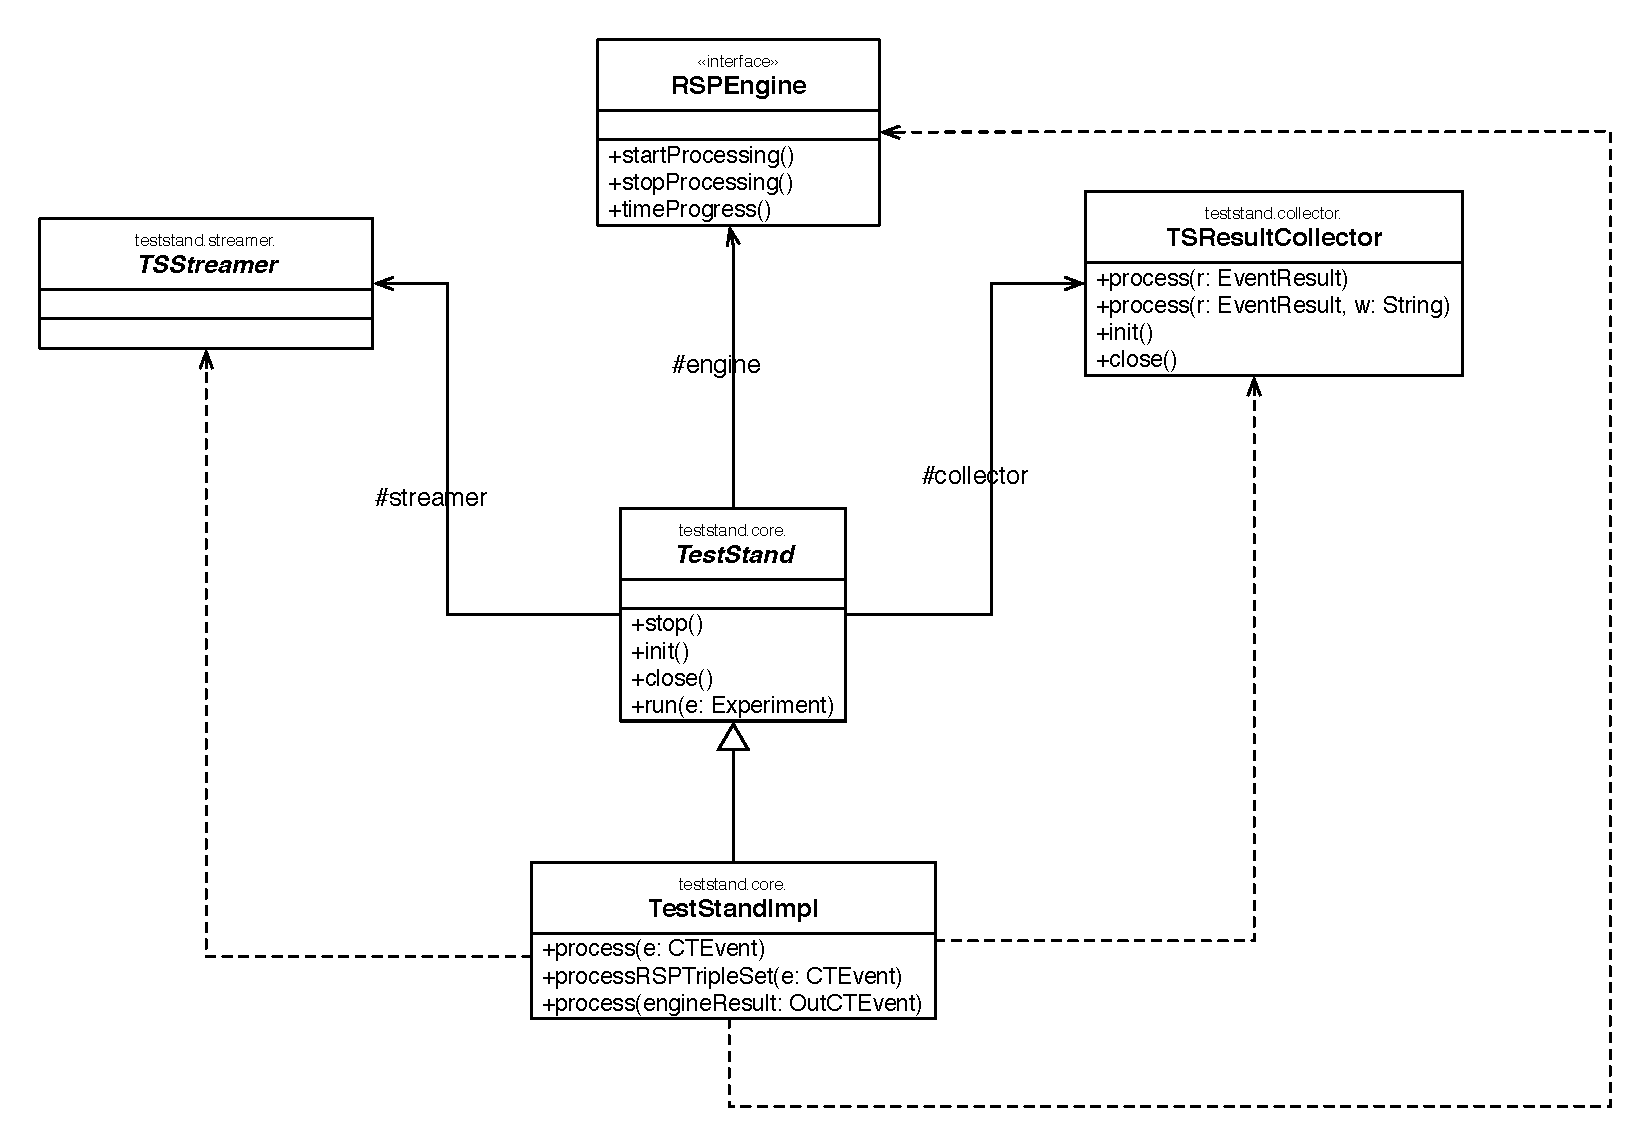
\includegraphics[width=0.90\linewidth]{images/uml_teststand_modules}
	\caption{UML Schema the TestStand with the upstanding modules: TSStreamer, RSPEngine, TSResultCollector} 
  	\label{fig:uml_teststand_modules}
\end{figure}

During the execution \textit{TestStandImpl} intercepts the \textit{CTEvents} form the \textit{TSStreamer} and sends them to the \textit{RSPEngine} as described in Section \ref{sec:arch-workflow}. According with the \textit{Experiment} specification the \textit{TestStandImpl} turns off or on its sensors. It calculates latency starting a timer when the \textit{CTEvent} arrives and stops the timer when it \textit{RSPEngine} outputs the results. It retrieves the memory usage asking the JVM in both the point above [R.6]. To fulfil requirements [R.7] any new measurement can take place  when the \textit{RSPEngine} is not running yet or when it has finished the computation. Once the \textit{OutCTEvents} comes form the \textit{RSPEngine}, the \textit{TestStandImpl} receives it and wraps it within a \textit{TSResult}, then it sends the query results data together with the measures to the \textit{TSResultCollector} fulfilling [R.8] and supporting [R.9] for further analysis with the Analyser.
%
%R.6 include basic set of performance measurements [?].
%R.7 enable users extensions with new software sensors and specific measure-
%ments collection.
%R.8 support performance measurements collection for further analysis.

\section{Baselines}\label{sec:baselines-impl}

\name Baselines are four elementary implementation of an RSP Engine which follow the design proposal presented in Section \ref{sec:baselines}, covering [R.13]. They pipeline Esper\footnote{$http://www.espertech.com/esper/$}, a mature commercial DSMS, with the Jena general purpose rule engine\footnote{http://jena.apache.org/documentation/inference/\#rules
}, a flexible reasoning engine. The motivations behind the choice of Esper and Jena regards the intention to fulfil requirement [R.14], baselines Eligibility, coupling this two good solution for reasoning and CEP, to obtain a fair solution the SR context. 

\begin{figure}[tbh]
  \centering
	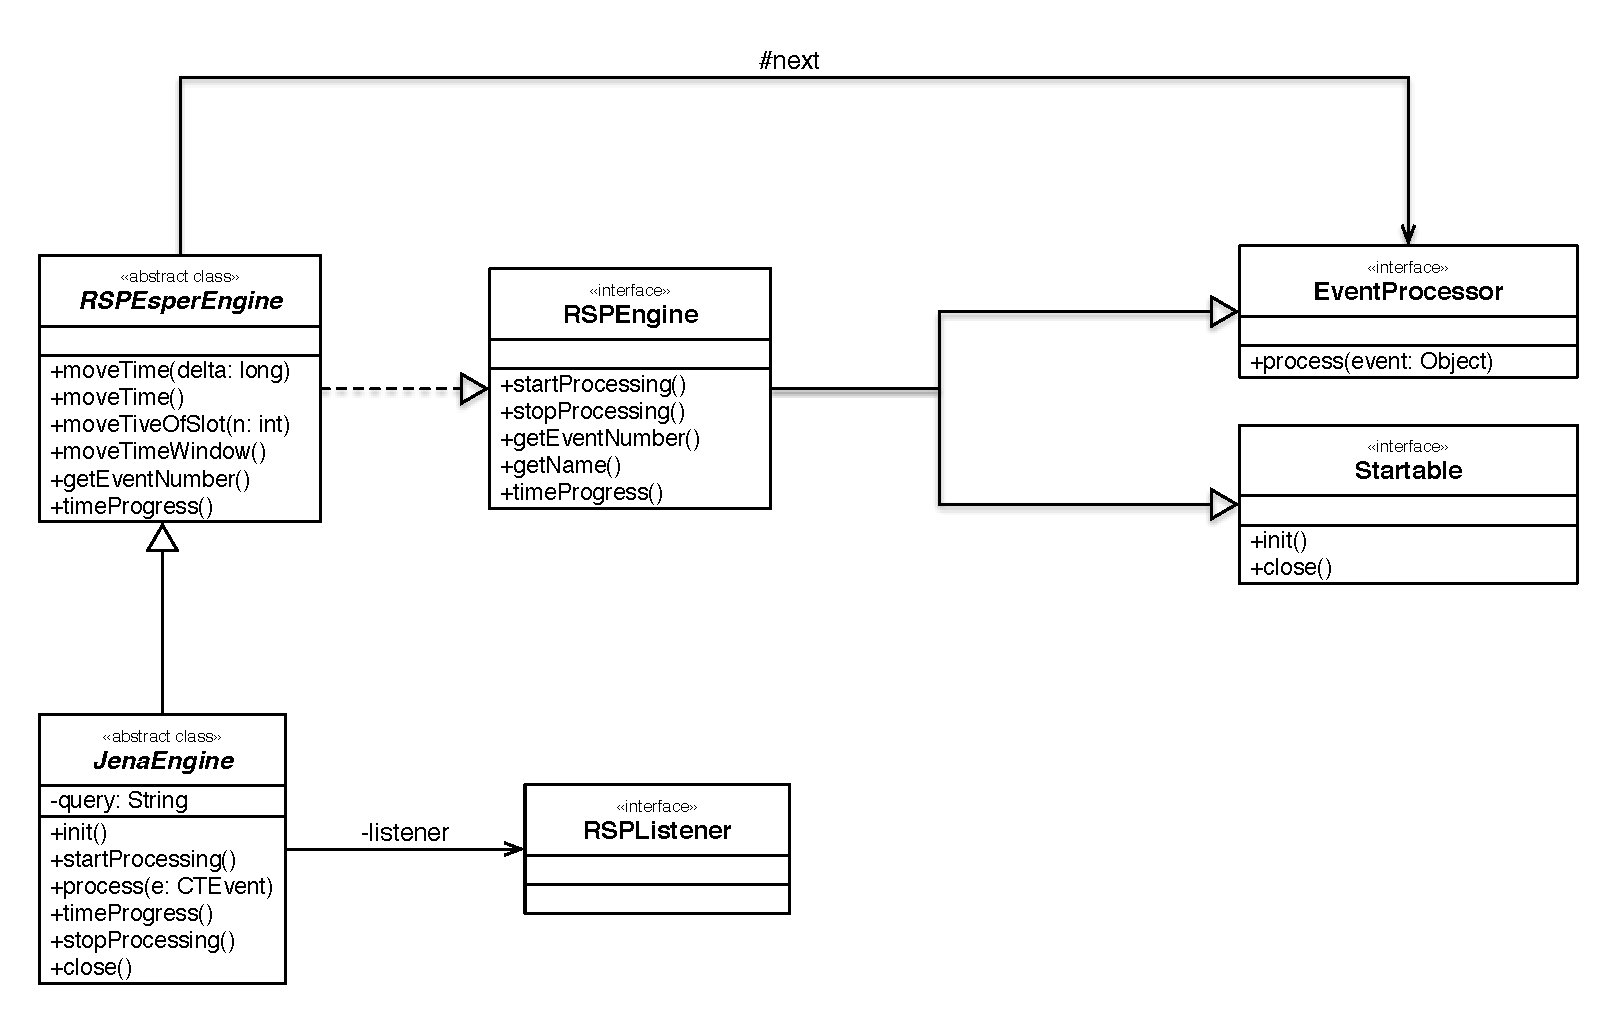
\includegraphics[width=\linewidth]{images/uml_baselines_general}
	\caption{RSPEsper Engine General UML Schema} 
  	\label{fig:uml_baselines_general}
\end{figure}

Figure \ref{fig:uml_baselines_general} shows the general implementation of the baselines: they  exploit the \textit{RSPEngine} interface, a proxy for an \textit{EventProcessor}, implementing the interface into the \textit{RSPEsperEngine} abstract class that includes the esper runtime.  The proposed baselines take advantage of the ability of esper to be temporally controlled by an external agent\footnote{\url{http://esper.sourceforge.net/esper-0.7.5/doc/reference/en/html_single/index.html#api-controlling-time}} by sending time-keeping events to synchronise the internal time flow. One time-keeping event is sent before injecting the triples within a \textsc{CTEvent} and another one after all triples in \textsc{CTEvent} were sent. In this way all the triples in the \textsc{CTEvent} are consider contemporary by the baselines. To enable external time control the RSPEngine interface exposes the moveTime() method, whose implementation depends on the particular RSP Engine in use. The next attributes, represents the general \textit{EventProcessor} which follows the RSPEngine in the \textsc{Test Stand} pipeline, it can be any modules which processes \textit{CTEvent}.

\begin{figure}[tbh]
  \centering
	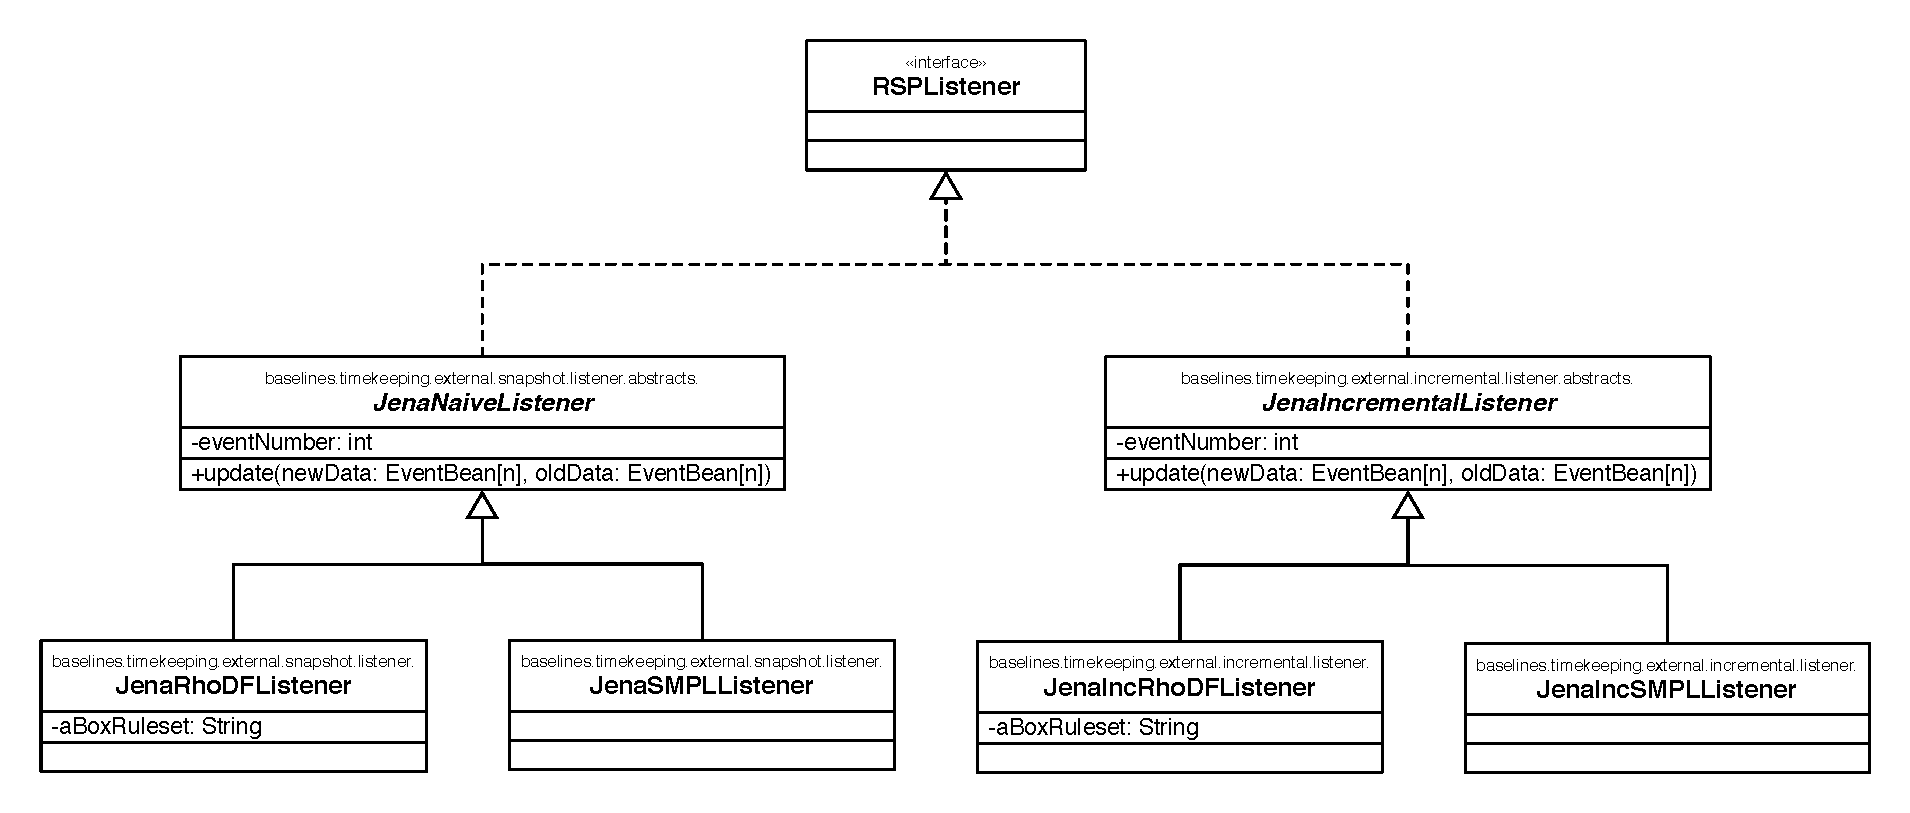
\includegraphics[width=\linewidth]{images/uml_baselines_listener}
	\caption{RSPListener UML Schema} 
  	\label{fig:uml_baselines_listener}
\end{figure}

In Figure \ref{fig:uml_baselines_general} is visible also the interaction between  the RSP Engine, represented by \textit{JenaEngine} abstract class, with the incoming \textit{CTEvent}. The engine is referencing the \textit{RSPListener} responsible to pipeline the Jena rule engine to the DSMS. 

\begin{figure}[tbh]
  \centering
	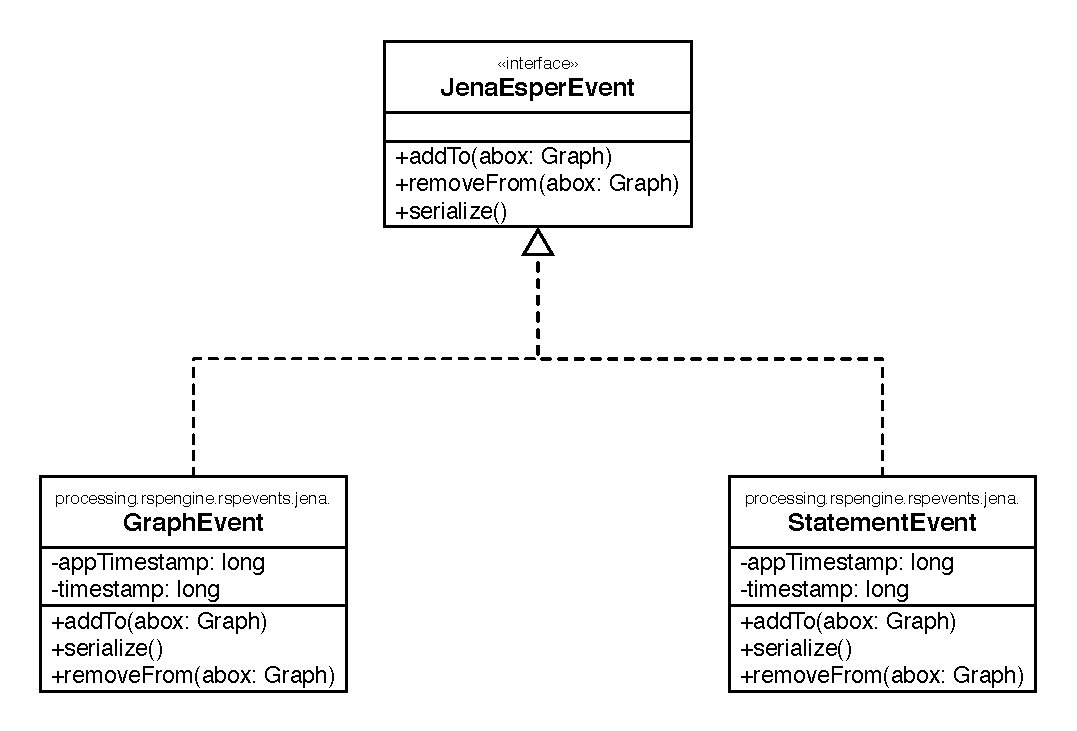
\includegraphics[width=0.5\linewidth]{images/uml_baselines_events}
	\caption{Esper-level events UML Schema} 
  	\label{fig:uml_baselines_events}
\end{figure}

Figure \ref{fig:uml_baselines_listener} shows the different implementations of the \textit{RSPListener}, which specify the reasoning approaches, Naive or Incremental as demanded by [R.15] (baseline relevance), according with the baseline design presented in Section \ref{sec:baselines}. Neither the \textit{JenaNaiveListener} or the \textit{JenaIncrementalListener} specify the entailment regime, which must be defined with specific implementations as it is visible in the Figure.\\

\pagebreak

When a \textit{CTEvents} comes to the RSP Engine it will be transformed into the events handled by the DSMS, \ref{fig:uml_baselines_events}, this translation process influence the latency calculus. Once the processing is complete, the output of the RSP Engine is injected into an \textit{OUTCTEvent} and passed to the next \textit{EventProcessor} in the pipeline, which is the \textsc{Test Stand}. \textit{JenaEsperEvent} interface, as reported in Figure \ref{fig:uml_baselines_events} exposes methods to interact with the RDF model, independently from the event implementation. The figure shows the current two implementation, Graph Based or Triple Based, which cover again [R.15] about baseline Relevance. Moreover, Figure \ref{fig:uml_baselines_rel_listener_event} shows how the \textit{JenaNaiveListener} and the  \textit{JenaIncrementalListener} handles the events which come form the DSMS trough the \textit{JenaEsperEvent} interface, for the case of Graph-based event representation (see Section \ref{sec:baselines} for event details). 

\begin{figure}[tbh]
  \centering
	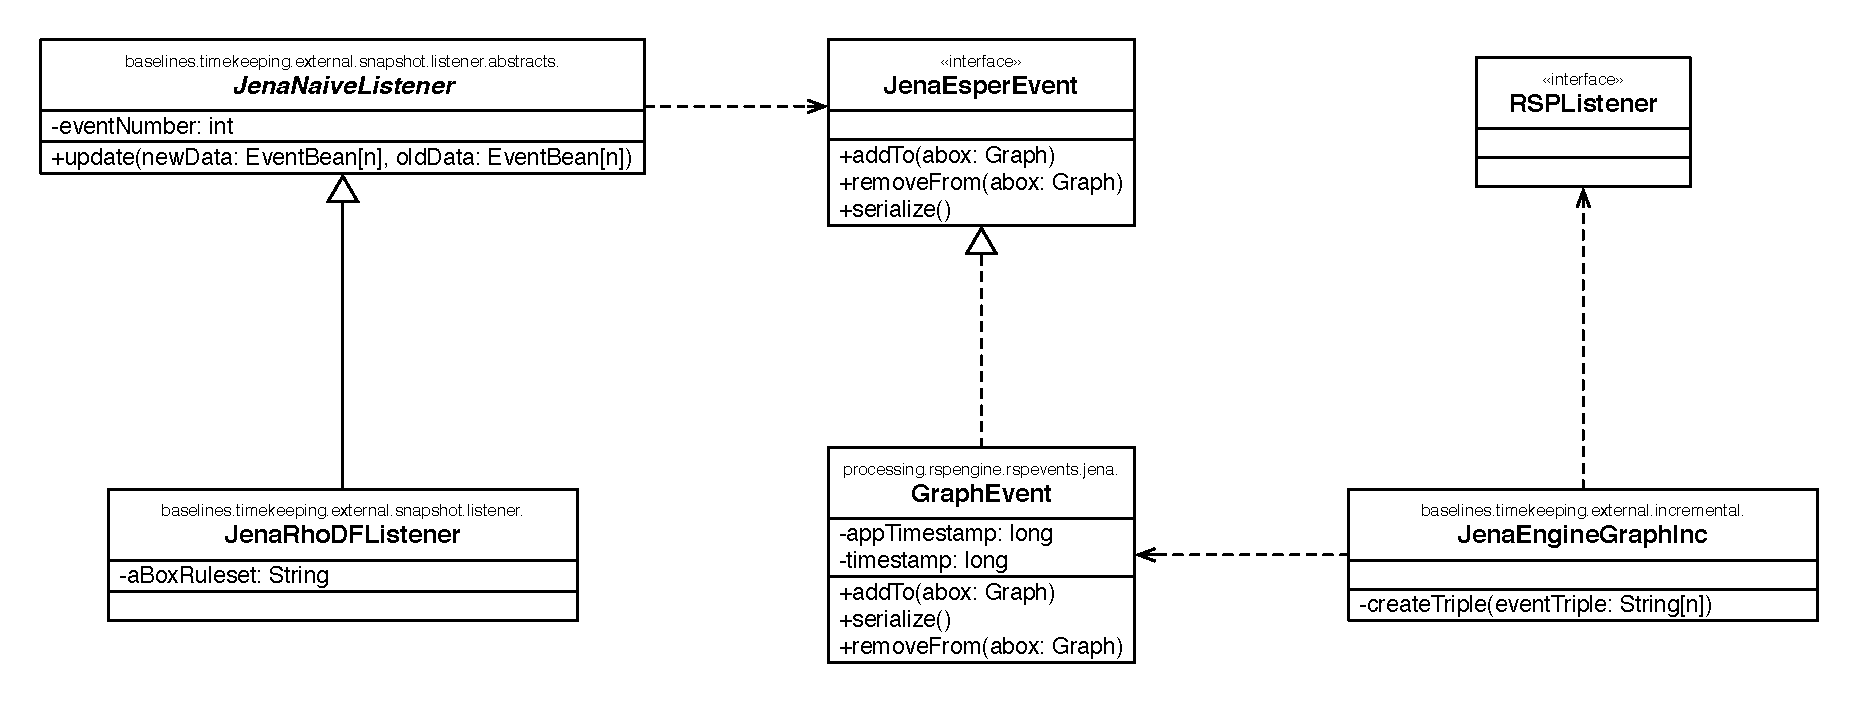
\includegraphics[width=\linewidth]{images/uml_baselines_rel_listener_event}
	\caption{RSPListener and events UML Schema} 
  	\label{fig:uml_baselines_rel_listener_event}
\end{figure}

This design allow the baselines to have a common design, sharing the majority of the code by splitting the different architectural elements. In this way we fulfil [R.16] which demands baseline Simplicity.


\section{Analyser}\label{sec:analyser-impl}

%R.9 allow qualitative analysis trough tools for result visualization



